\chapter{Diseño e Implementación} % Main chapter title

\label{Chapter3} % Change X to a consecutive number; for referencing this chapter elsewhere, use \ref{ChapterX}
\definecolor{mygreen}{rgb}{0,0.6,0}
\definecolor{mygray}{rgb}{0.5,0.5,0.5}
\definecolor{mymauve}{rgb}{0.58,0,0.82}

\lstset{ %
  backgroundcolor=\color{white},   % choose the background color; you must add \usepackage{color} or \usepackage{xcolor}
  basicstyle=\footnotesize,        % the size of the fonts that are used for the code
  breakatwhitespace=false,         % sets if automatic breaks should only happen at whitespace
  breaklines=true,                 % sets automatic line breaking
  captionpos=b,                    % sets the caption-position to bottom
  commentstyle=\color{mygreen},    % comment style
  deletekeywords={...},            % if you want to delete keywords from the given language
  %escapeinside={\%*}{*)},          % if you want to add LaTeX within your code
  %extendedchars=true,              % lets you use non-ASCII characters; for 8-bits encodings only, does not work with UTF-8
  %frame=single,	                   % adds a frame around the code
  keepspaces=true,                 % keeps spaces in text, useful for keeping indentation of code (possibly needs columns=flexible)
  keywordstyle=\color{blue},       % keyword style
  language=[ANSI]C,					% the language of the code
  %otherkeywords={*,...},           % if you want to add more keywords to the set
  numbers=left,                    % where to put the line-numbers; possible values are (none, left, right)
  numbersep=5pt,                   % how far the line-numbers are from the code
  numberstyle=\tiny\color{mygray}, % the style that is used for the line-numbers
  rulecolor=\color{black},         % if not set, the frame-color may be changed on line-breaks within not-black text (e.g. comments (green here))
  showspaces=false,                % show spaces everywhere adding particular underscores; it overrides 'showstringspaces'
  showstringspaces=false,          % underline spaces within strings only
  showtabs=false,                  % show tabs within strings adding particular underscores
  stepnumber=1,                    % the step between two line-numbers. If it's 1, each line will be numbered
  stringstyle=\color{mymauve},     % string literal style
  tabsize=2,	                   % sets default tabsize to 2 spaces
  title=\lstname,                   % show the filename of files included with \lstinputlisting; also try caption instead of title
  morecomment=[s]{/*}{*/}%
}


%----------------------------------------------------------------------------------------
%	SECTION 1
%----------------------------------------------------------------------------------------
En este capítulo se veremos cómo se desarrolló un hardware básico para poder simular el entorno de funcionamiento y cómo fue implementado el firmware.
%La idea de esta sección es resaltar los problemas encontrados, los criterios utilizados y la justificación de las decisiones que se hayan tomado.
%Se puede agregar código o pseudocódigo dentro de un entorno lstlisting con el siguiente código:

\section{Hardware}

Se diseño de un circuito, que permite simular el entorno de funcionamiento de una bodega. Para ello se utilizó lo aprendido a la largo del curso de \emph{diseño de PCBs en KICAD}. Si bien, por falta de tiempo, no se llevo a cabo el desarrollo de la placa diseñada que veremos a , a fines de poder testear el sistema se elaboro una versión simplificada. 

Surgieron varios imprevistos, principalmente con el modulo SIM800L, el cual posee grandes inconvenientes a la hora de detectar la SIM. Luego de una serie de búsquedas en internet, donde muchos habían tenido un problema similar debido a:
\begin{itemize}
  \item Fuente de alimentación subdimensionada.
  \item Modulo muy sensible, limpiar bien los contactos de la SIM.
  \item Problemas en la soldadura del módulo.
\end{itemize}
Finalmente, si bien dicho modulo ya había sido comprado y se encontró la falla a tiempo se utilizó en el prototipo, pero este no se recomienda. Ya que trae consigo los problemas mencionados anteriormente.. A futuras implementación este módulo será reemplazado.


\subsection{Diagrama en bloque}
En el siguiente esquema, Figura \ref{fig:diagrama_sistema} podemos apreciar el entorno de trabajo del dispositivo. Donde el mismo   interactuar con una bomba de agua que permite llevar desde el deposito del liquido refrigerante a los tanques que están en proceso de fermentación.
Recibiendo como información la temperatura de los tanques, este debe controlar la bomba y la electroválvula correspondiente. De esta forma permitirá tener controlada la temperatura acorde a los parámetros definidos por el usuario. 


\begin{figure}[!htb]
  \centering
  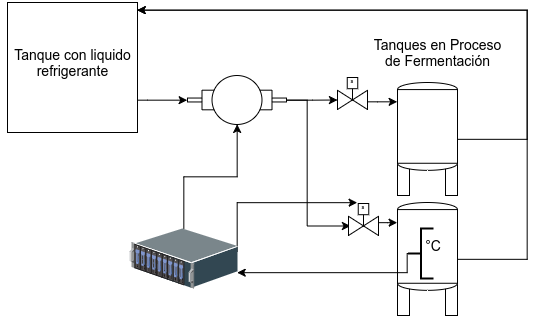
\includegraphics[scale=0.3]{./Figures/diagrama_del_sistema.png}
  \caption{Esquema de interacción del dispositivo.}
  \label{fig:diagrama_sistema}
\end{figure}

\subsection{ Módulos requeridos}
Para llevar a cabo el proyecto, se dividió el sistema en los siguientes módulos:
\begin{description}
  \item[Módem:] sera el encargado de transmitir las alertas mediante SMS utilizando el modulo SIM800L.
  \item[Actuadores:] salidas que nos permiten controlar la bomba y electroválvulas. Debido a que se utilizo la CIA-NXP ya esta resuelto.
  \item[Sensores:] entradas que permitan simular el comportamiento de los sensores, para esto se utilizaron potenciómetros.
  \item[CPU:] unidad encargada de controlar el funcionamiento del sistema. Incorporada en la placa CIA-NXP. 
\end{description}

Con lo cual podemos ver que el CPU y los actuadores ya están desarrollados al haber elegido la CIA. Nos quedara ver los sensores y el módem en la próxima sección.

\subsection{Características del hardware}
El sistema cuenta con:

\begin{itemize}
  \item 1 Salida con regulación de corriente, para simular sensores de 4mA a 20mA.
  \item 1 Salida con tensión variable, utilizando el regulador LM317.
  \item 1 Salida del sensor de temperatura LM35.
  \item 2 Salidas con tensión variable, utilizando potenciómetros. 
  \item 4 Entradas digitales conectadas a leds.
  \item 4 Salidas conectadas a pulsadores. 
  \item 1 Zócalo para la conexión del modulo SIM800L. 
  \item 1 salida de 5V a 3A y otra de 3.3V a 1A. 
\end{itemize}

El módulo SIM800l que se muestra en la siguiente Figura \ref{fig:sim800l}, es un módem GPRS que cuenta con las siguientes especificaciones:

\begin{figure}[!htb]
  \centering
  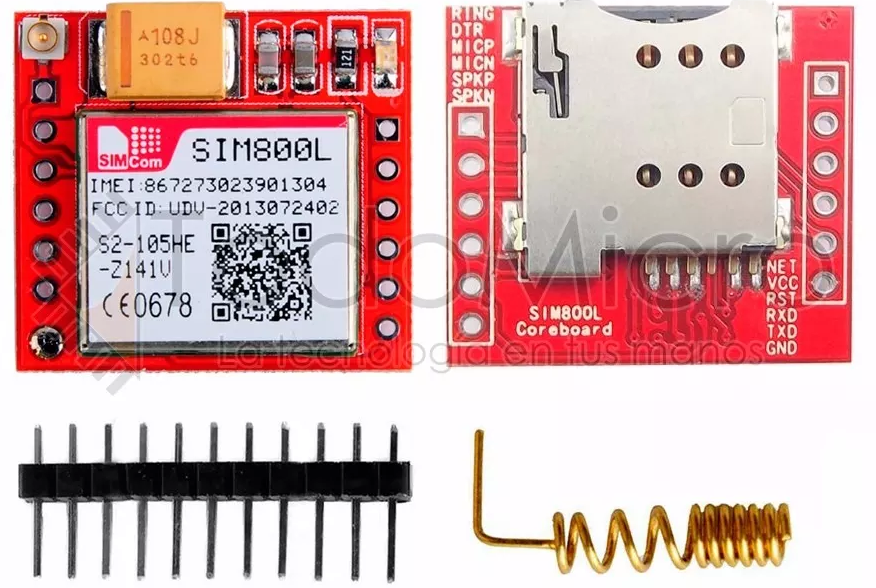
\includegraphics[scale=0.2]{./Figures/sim800.png}
  \caption{Módem SIM800L.}
  \label{fig:sim800l}
\end{figure}

\begin{itemize}
  \item Alimentación: 3.4V a 4.4V (4.0V recomendado)
  \item  CuatriBanda 850/900/1800/1900MHz
  \item  GPRS Multi Slot class 8/10
  \item  Control mediante comandos AT (GSM 07.07 ,07.05 y comandos AT SIMCOM).
\end{itemize}


En la figura \ref{fig:essim800} se puede apreciar el esquemático implementado para la conexión del módem GSM. Éste requiere adaptar los niveles de tensión para interactuar con la CIA-NXP, para el cual utilizamos un max3232.
\begin{figure}[!htb]
  \centering
  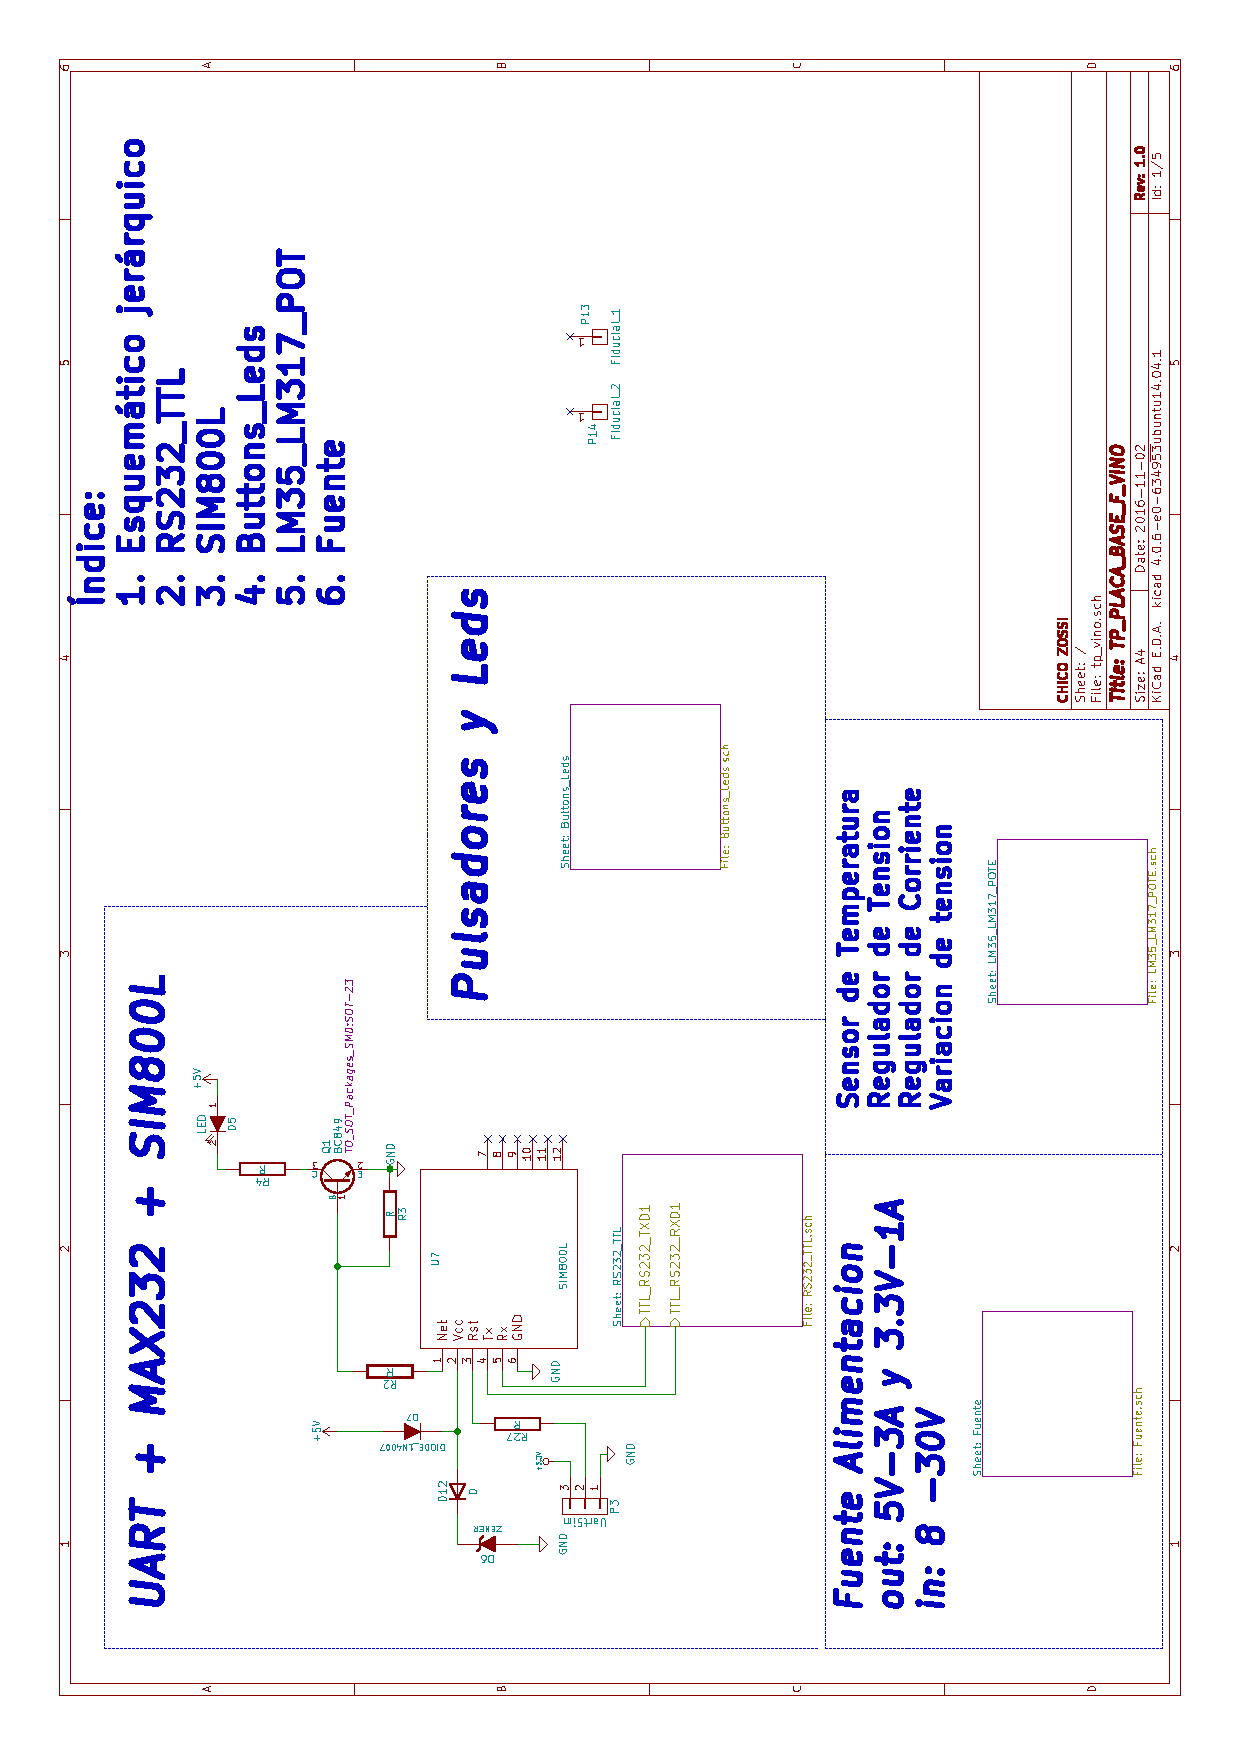
\includegraphics[page=1,scale=0.3,angle=270]{./Figures/schematic.pdf}
  \caption{Módulo SIM800l e índice de esquemáticos.}
  \label{fig:essim800}
\end{figure}

Para la alimentación del circuito se utilizó el regulador LM2576. El mismo se tomó de la nota de aplicación el diagrama típico.\footnote{Nota de aplicación Texas Instruments: \url{http://www.ti.com/lit/ds/symlink/lm2576.pdf}}
Para regular a 3.3V se utilizó el integrado LM11733 circuito extraído de la nota de aplicación. \footnote{ Texas Instruments: \url{http://www.ti.com/lit/ds/symlink/lm1117.pdf} - Capitulo 8 Figura 16 } 
\begin{figure}[!htb]
  \centering
  \includegraphics[page=3,scale=0.3,angle=270]{./Figures/schematic.pdf}
  \caption{Fuente de alimentación DC/DC.}
  \label{fig:fuente}
\end{figure}

Para lograr la simulación de distintos tipos de sensores, se utilizaron circuitos como se muestra en la figura \ref{fig:temp_tens}  que permiten generar corrientes 4mA a 20mA, variaciones de la tensión, y hasta un sensor de temperatura. Para los circuitos se utilizaron las notas de aplicación de Texas Instruments\footnote{Reguladores de Tensión y Corriente \url{http://www.ti.com/lit/ds/symlink/lm317.pdf} - capitulo 8 páginas 12 y 13 y sensor temperatura: \url{http://www.ti.com/lit/ds/symlink/lm35.pdf} - 8.2.1 Basic Centigrade Temperature Sensor } 
\begin{figure}[!htb]
  \centering
  \includegraphics[page=4,scale=0.3,angle=270]{./Figures/schematic.pdf}
  \caption{Regulador de corriente, de tensión y del sensor de temperatura.}
  \label{fig:temp_tens}
\end{figure}

Para concluir, se utilizaron unos circuitos básicos que permiten interactuar en forma simple con el sistema y realizar pruebas de funcionamiento. Los mismos fueron extraídos del esquemático utilizado en el proyecto de la EDU-CIA\footnote{\url{http://www.proyecto-ciaa.com.ar/devwiki/lib/exe/fetch.php?media=desarrollo:edu-ciaa:edu-ciaa-nxp:edu-ciaa-nxp\_color.pdf}}

\begin{figure}[!htb]
  \centering
  \includegraphics[page=5,scale=0.3,angle=270]{./Figures/schematic.pdf}
  \caption{Entradas a leds y salidas de los pulsadores.}
  \label{fig:pul_leds}
\end{figure}

Una vez realizados los esquemáticos, se pasó a la elaboración del PCB. Se realizaron los ruteo necesarios. Y como se puede observar en la siguientes figuras \ref{fig:layer_sup} - \ref{fig:layer_inf} 
\begin{figure}[!htb]
  \centering
  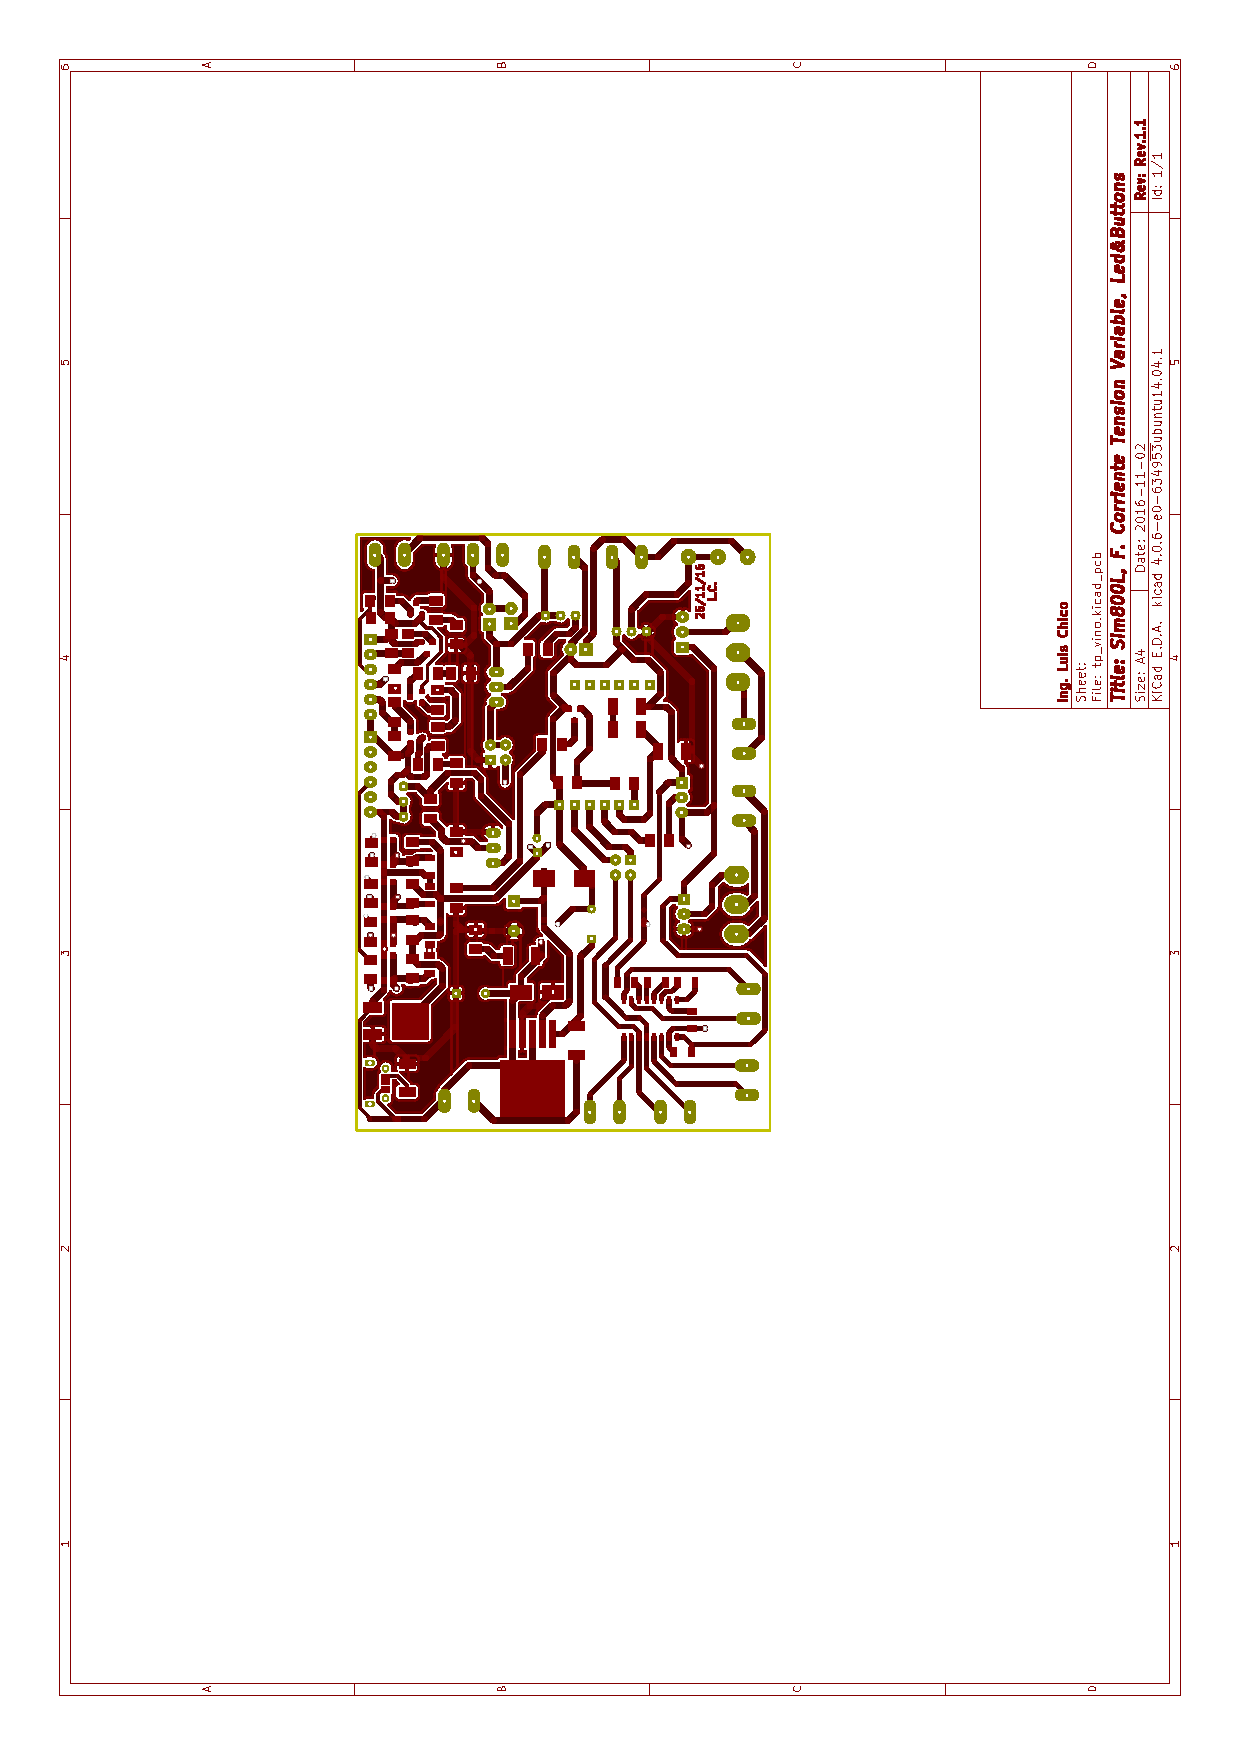
\includegraphics[page=1,angle=270,clip,trim=5.5cm 10cm 7.7cm 8.5cm]{./Figures/pcb_layer.pdf}
  \caption{Capa superior de la placa simulador de sensores.}
  \label{fig:layer_sup}
\end{figure}
\begin{figure}[!htb]
  \centering
  \includegraphics[page=2,angle=270,clip,trim=5.5cm 10cm 7.7cm 8.5cm]{./Figures/pcb_layer.pdf}
  \caption{Capa inferior de la placa simulador de sensores.}
  \label{fig:layer_inf}
\end{figure}

Realizando una vista previa de como quedaría el esquema y aprovechando el potencial de la herramienta de KICAD, se realizó una vista 3D de como quedaría, la que se puede apreciar en la figura \ref{fig:pcb3d}.

\begin{figure}[!h]
  \centering
  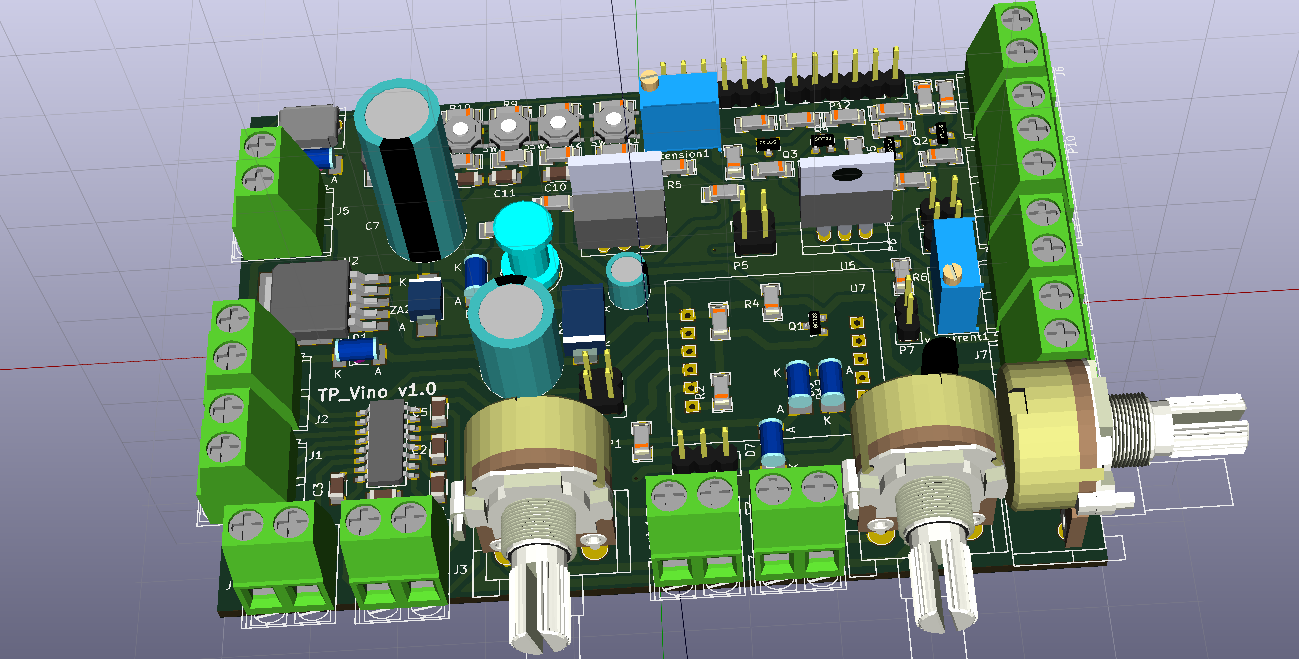
\includegraphics[scale=0.3]{./Figures/pcb_3d.png}
  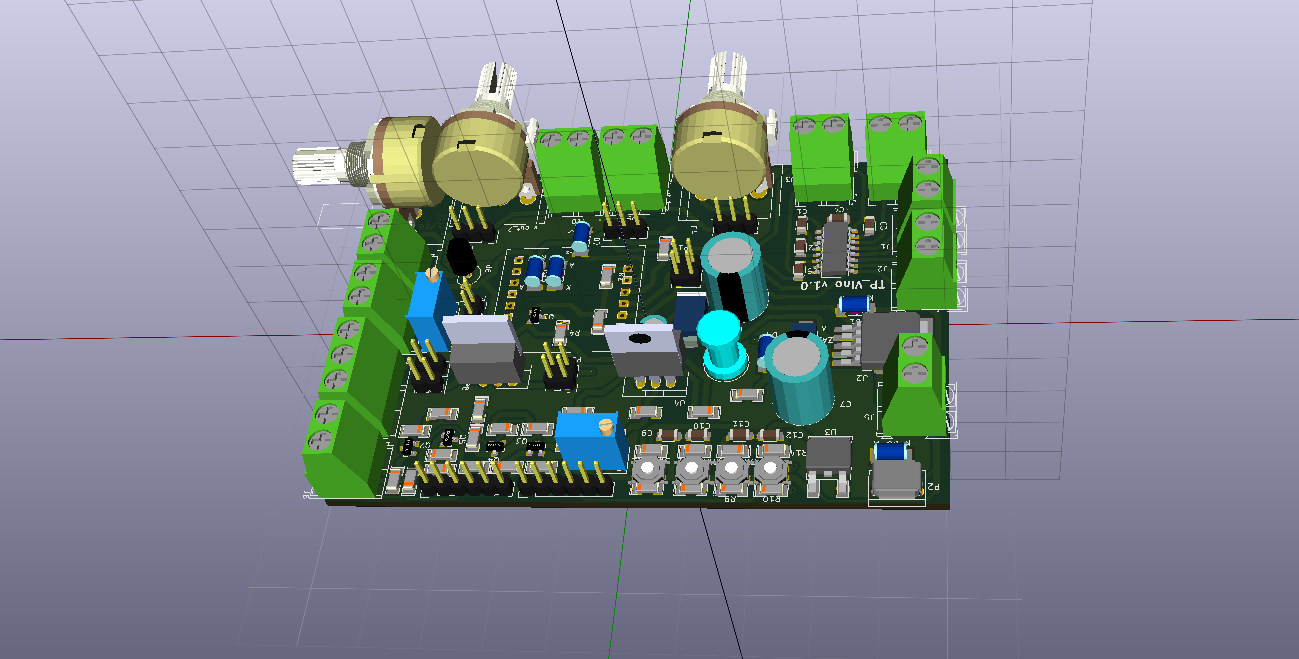
\includegraphics[scale=0.3]{./Figures/pcb_3d_back.png}
  \caption{Placa simulador de sensores 3D.}
  \label{fig:pcb3d}
\end{figure}

No obstante, por cuestiones de tiempo no se llegó a implementar. Simplemente quedó en una primera etapa para una posterior implementación. Se terminó desarrollando una placa experimental que permitió realizar las primeras pruebas. Podemos verla en la siguiente figura \ref{fig:placa_básicafirst}

\begin{figure}[!h]
  \centering
  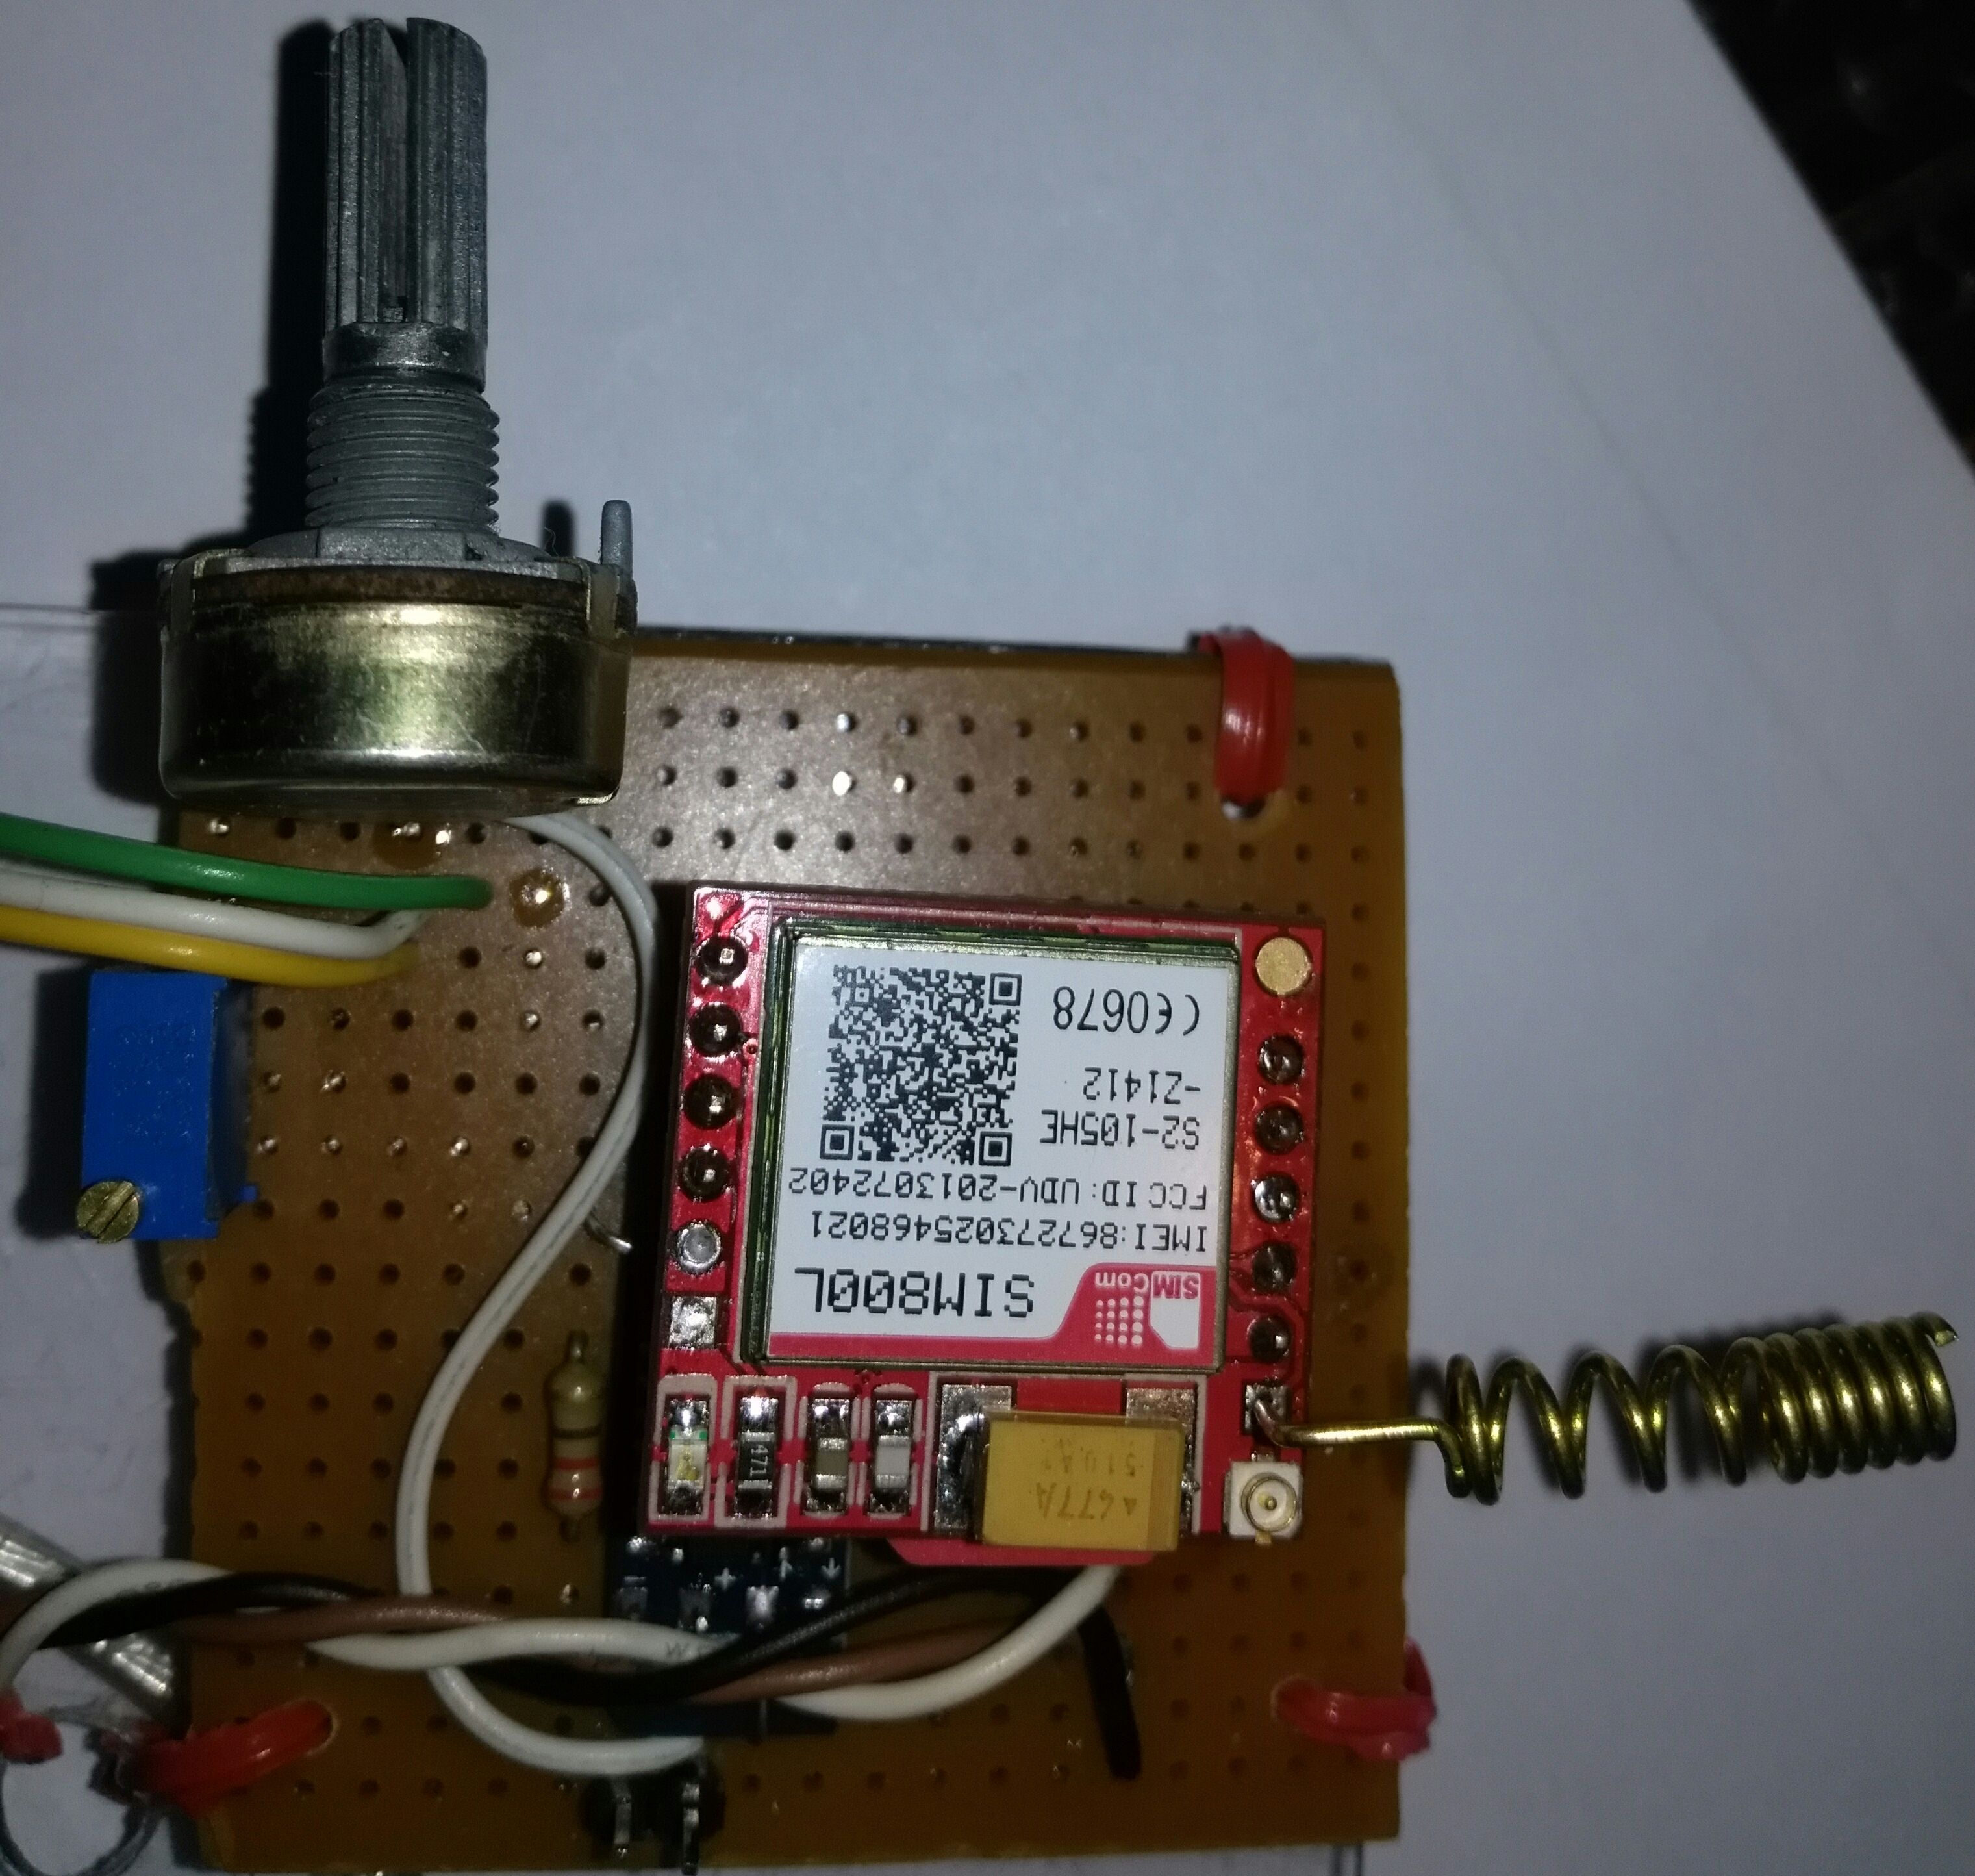
\includegraphics[scale=.03]{./Figures/placa_basica.jpg}
  \caption{Placa de simulación de temperatura y estado de la batería con el modulo SIM800l integrado.}
  \label{fig:placa_básicafirst}
\end{figure}


\section{Software}
\subsection{Aplicación}
Se dividieron las tareas por recursos:
\begin{itemize}
  \item Módem 
  \item Control
  \item Sensores
\end{itemize}

\subsection*{Módem}
En esta tarea se inicializa las configuraciones iniciales para el uso del módem. Es la encargada de interactuar con el módulo GPRS, realizando consultas del estado de señal y de enviando los mensajes de alarmas en caso de ser necesarios.

Podemos ver como fue implementado en el diagrama de flujo en la siguiente figura \ref{fig:modem_task}.

\begin{figure}[!htb]
  \centering
  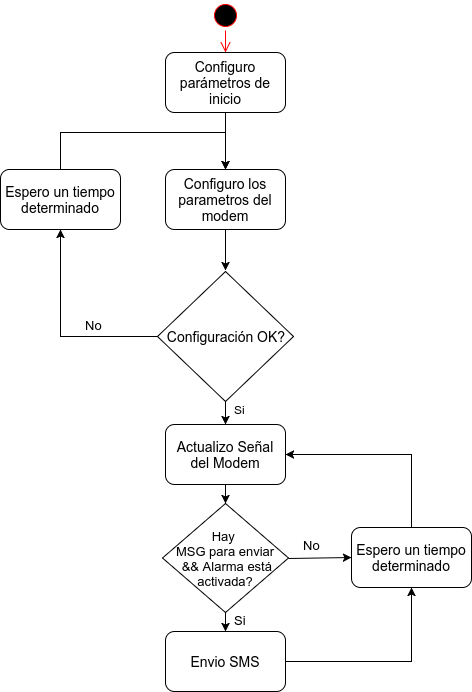
\includegraphics[scale=.5]{./Figures/modem_task.png}
  \caption{Diagrama de flujo de la tarea que controla el módem GPRS.}
  \label{fig:modem_task}
\end{figure}


\subsection*{Control}
Con esta tarea se analiza el resultado los sensores de temperatura, y de la batería. Se verifica que estén dentro de los parámetros configurados por el usuario y se actúa en consecuencia.

También es la encargada de setear los actuadores según sean especificados en la plataforma web.

La implementación se puede apreciar en la siguiente figura \ref{fig:control_task}.

\begin{figure}[!htb]
  \centering
  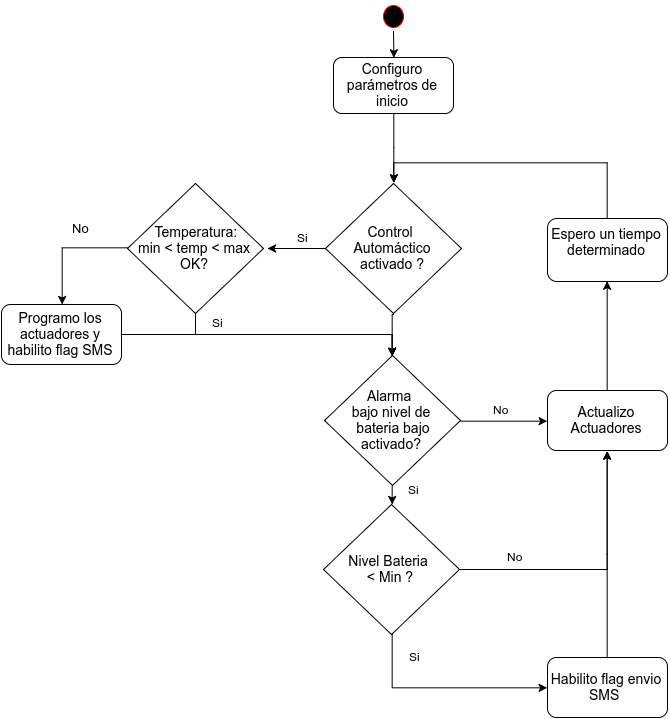
\includegraphics[scale=.5]{./Figures/control_task.png}
  \caption{Diagrama de flujo de la tarea de control.}
  \label{fig:control_task}
\end{figure}


\subsection*{Sensor}
 En este caso la tarea es más simple, consulta el estado de los sensores y calcula el promedio de las ultimas N muestras, este es el valor que usa el control para definir si es necesario encender los actuadores correspondientes.

 Como vemos en el siguiente diagrama de flujo, figura \ref{fig:sensor_task}.

\begin{figure}[!htb]
  \centering
  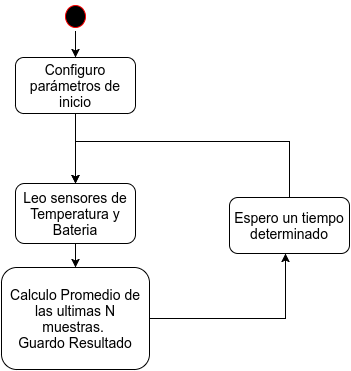
\includegraphics[scale=.5]{./Figures/sensor_task.png}
  \caption{Diagrama de flujo del sensor.}
  \label{fig:sensor_task}
\end{figure}

\subsection{Web}
Mediante la plataforma web diseñada se busca que el usuario pueda ver los datos de los sensores, tener control sobre los actuadores y realizar las configuraciones necesarias. 

Para poder realizarlo, fue necesario profundizar los siguientes temas:
\begin{description}
    \item[HTML:] En dicho código se desarrollo la página web, este permite darle la estructura básica y se realiza sobre texto plano, es decir no se requiere ninguna aplicación adicional simplemente un editor de texto. Luego es el navegador web quien tiene la tarea de interpretarlo. 
    \item[CSS:] Mediante este código se realiza la presentación de la página, permitiendo así modificar la visualización de la misma y darle un formato mas profesional y elegante.
    \item[SVG:] Mediante este código se implementaron los gráficos correspondientes para mostrar los resultados de los sensores y el estado de los actuadores.
    \item[AJAX:] es un recurso muy utilizado para cuando de desarrollan web en sistemas embebidos. Permite actualizar el estado de la web sin tener que consultar todo el contenido, simplemente se descarga una primera vez y luego se puede realizar consultar los valores que quieren actualizar. 
    \item[SSI:] Si bien la implementación que nos ofrece FreeRTOS es reducida. Es más que suficiente para poder agregar contenido a nuestra pagina en forma dinámica.
    \item[CGI:] Por medio de este el cliente que navegar por nuestra plataforma puede enviar y solicitar datos, al servidor.
\end{description}

\subsection*{Diseño web}
Al iniciar el diseño de la web, no tenía experiencia previa. Es por ello que se inició buscando información en internet, varias páginas facilitaban algunos cursos de HTML, CSS, y AJAX  de forma online y gratuita. Las mas usadas fueron:
\begin{itemize}
  \item \url{https://www.w3schools.com}
  \item \url{https://es.khanacademy.org}
  \item \url{https://www.codecademy.com}
\end{itemize}
  con lo cual se logro una primera versión de la web, ver figura \ref{fig:old_web}.
\begin{figure}[!htb]
    \centering
    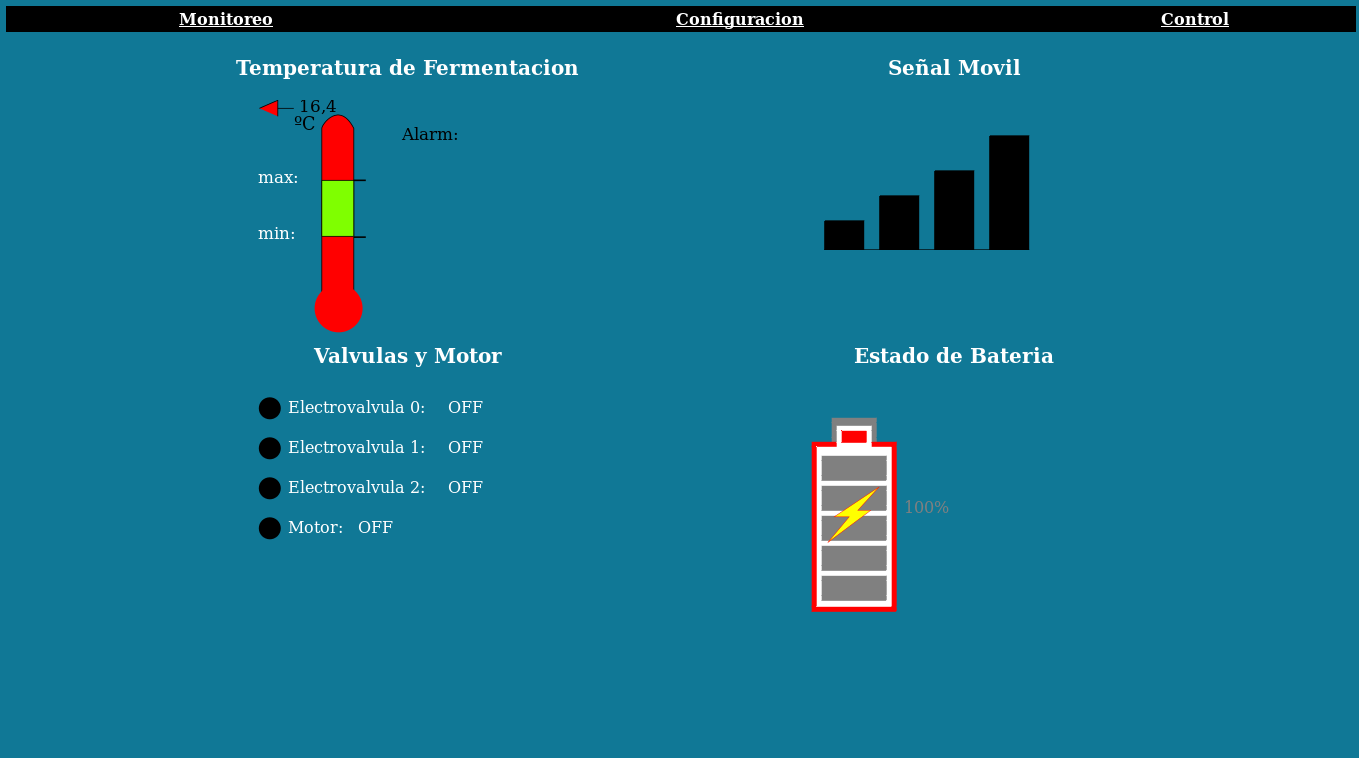
\includegraphics[scale=.25]{./Figures/old_web.png}
    \caption{Primera versión de la web de monitoreo.}
    \label{fig:old_web}
\end{figure}

Luego una vez que esta, estaba funcionando en forma correcta, se paso a mejorar las presentación de la misma, y para ello se usó un témplate que se ajustara a las necesidades, es decir mediante un archivo que contiene un estilo ya predefinido modifica la apariencia de la web. Pudiendo ver dicho cambio en la siguiente figura \ref{fig:web_monitoreo}.

\begin{figure}[!h]
  \centering
  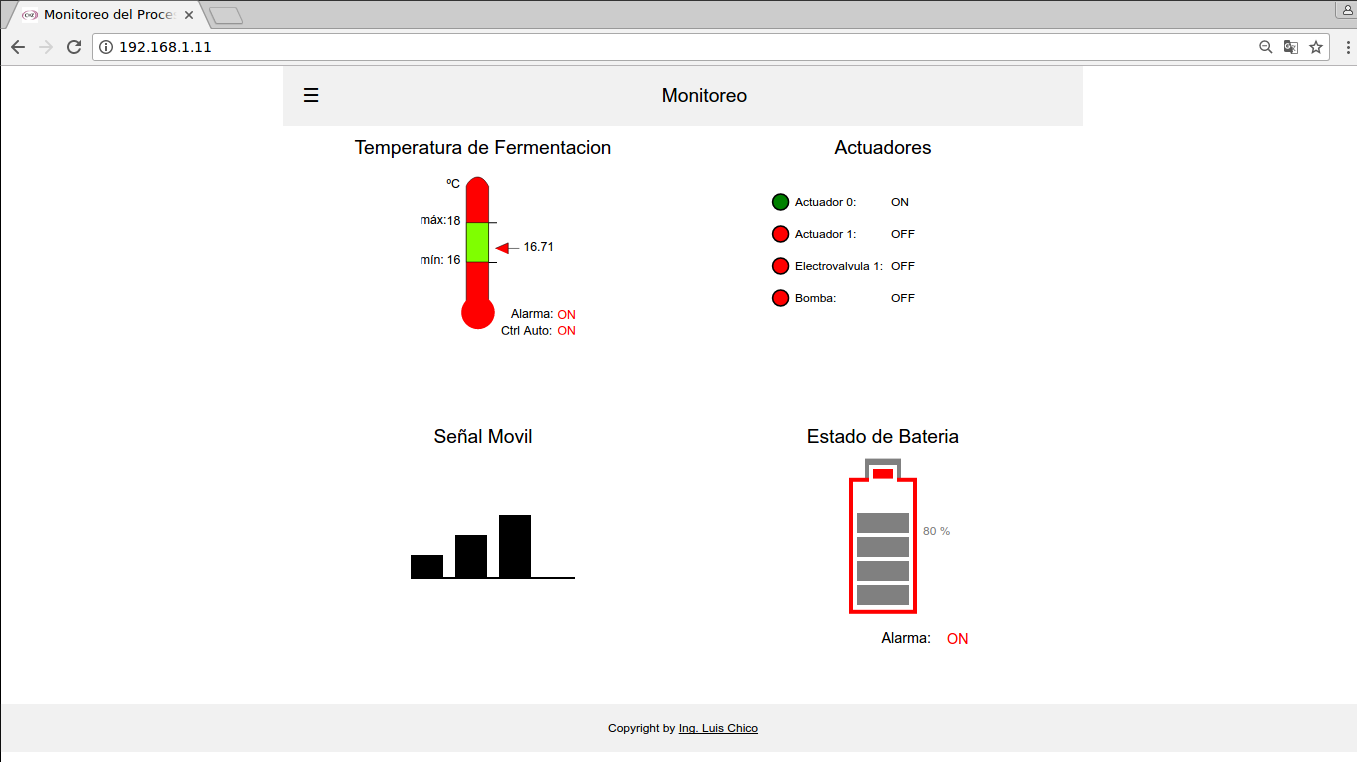
\includegraphics[scale=.25]{./Figures/web_monitoreo.png}
  \caption{Versión actualizada haciendo uso del témplate.}
  \label{fig:web_monitoreo}
\end{figure}

Este fue encontrando en w3school\footnote{\url{https://www.w3schools.com/w3css/w3css_templates.asp}}. Siendo que cumplía los siguientes requerimientos:
\begin{itemize}
  \item Sea amigable.
  \item Compatibles con distintos navegadores, especialmente los más utilizados como ser: Google-chrome y Firefox. 
  \item Sea cómodo de navegar en distintos dispositivos, como tablets, celulares y PCs.
\end{itemize}


\subsection*{Configuración del servidor}
Al iniciar el servidor debemos tener en cuenta que este sera el encargado de gestionar las peticiones del usuario. Es decir una vez que el usuario ingresa la dirección del servidor, este le transmite la información de la web.  Para realizar la comunicación entre cliente y servidor, se utilizo la API de lwIP  que utiliza una serie de callbacks para controlar los eventos debido a la comunicación de la red. Es por ello que para optimizar los recursos se utilizo AJAX, permitiendo que el cliente sea el encargado de realizar las consultas al server en forma periódica. La información se solicita mediante directivas del tipo SSI. Es decir, solo se transmite un archivo AJAX.shtml con los parámetros que se van a actualizar. Luego el navegador, mediante una serie de funciones en JavaScript es el encargado de actualizar los cambios realizados.  
Podemos ver el procedimiento mencionado den la siguiente figura\footnote{\url{http://laboratorios.fi.uba.ar/lse/tesis/LSE-FIUBA-Trabajo-Final-CESE-Patricio-Bos-2016.pdf}, figura 3.9.}:\ref{fig:ajax_sec} 
\begin{figure}[!htb]
    \centering
    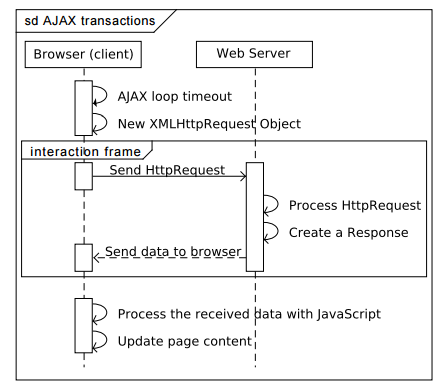
\includegraphics[scale=.8]{./Figures/ajax_sec.png}
    \caption{Diagrama de secuencia AJAX.}
    \label{fig:ajax_sec}
\end{figure}


La configuración establecida por default es la que se muestra en la siguiente Tabla \ref{tab:servercfg}.

\begin{table}[!h]
  \centering
  \begin{tabular}{l c}
    \hline 
    Parámetro    & Valor \\
    \hline \hline
    IP               & 192.168.1.11 \\
    Mascara de red   & 255.255.255.0 \\
    Puerta de enlace & 192.168.0.1 \\
    Puerto           & 80 \\
    DHCP             & Deshabilitado \\
    \hline
  \end{tabular}
  \caption{Configuración por default del servidor}
  \label{tab:servercfg}
\end{table}


%\begin{verbatim}
%\begin{lstlisting}[caption= "un epígrafe descriptivo"]
%
%	las líneas de código irían aquí...
%	
%\end{lstlisting}
%\end{verbatim}
%
%A modo de ejemplo:
%
%\begin{lstlisting}[caption=Pseudocódigo del lazo principal de control.]  % Start your code-block
%
%#define MAX_SENSOR_NUMBER 3
%#define MAX_ALARM_NUMBER  6
%#define MAX_ACTUATOR_NUMBER 6
%
%uint32_t sensorValue[MAX_SENSOR_NUMBER];		
%FunctionalState alarmControl[MAX_ALARM_NUMBER];	//ENABLE or DISABLE
%state_t alarmState[MAX_ALARM_NUMBER];						//ON or OFF
%state_t actuatorState[MAX_ACTUATOR_NUMBER];			//ON or OFF
%
%void vControl() {
%
%	initGlobalVariables();
%	
%	period = 500 ms;
%		
%	while(1) {
%
%		ticks = xTaskGetTickCount();
%		
%		updateSensors();
%		
%		updateAlarms();
%		
%		controlActuators();
%		
%		vTaskDelayUntil(&ticks, period);
%	}
%}
%\end{lstlisting}
%


